% -*- coding: UTF-8 -*-
% vim: autoindent expandtab tabstop=4 sw=4 sts=4 filetype=tex
% vim: spelllang=de spell
% chktex-file 27 - disable warning about missing include files

\section{Architektur}
\label{sec:architecture}

Die Architektur des~\hyperref[chap:prototype]{Prototypen} wurde bewusst einfach gehalten und ist
in~\autoref{fig:prototype_architecture} ersichtlich.

\begin{figure}[H]
    \centering
    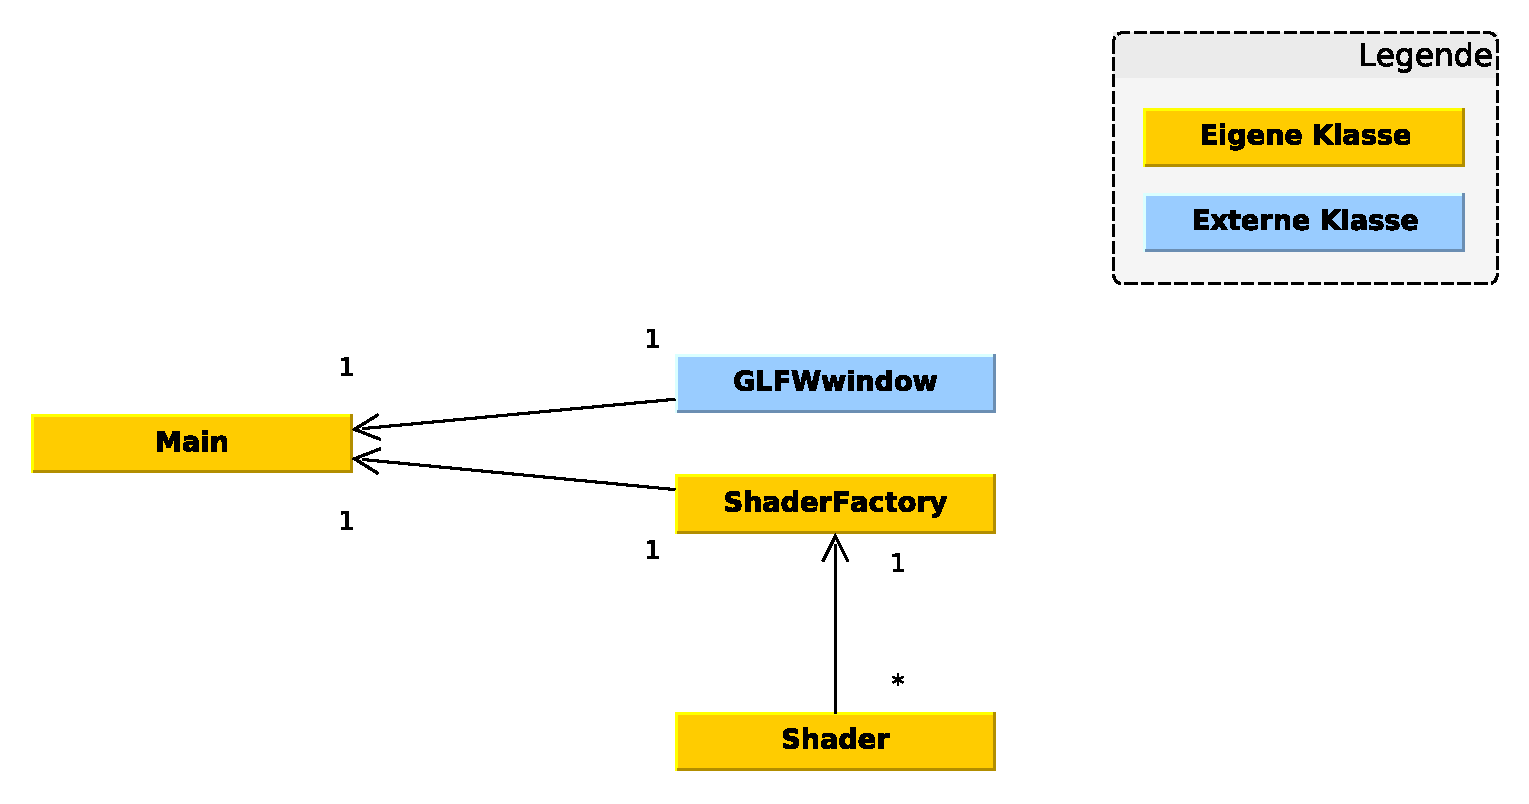
\includegraphics[width=0.8\textwidth]{img/prototype_class_diagram.pdf}
    \caption{Architektur des~\hyperref[chap:prototype]{Prototypen}\protect\footnotemark}\label{fig:prototype_architecture}
\end{figure}
\footnotetext{Eigene Darstellung mittels yEd.}

\subsection{Programmablauf}
\label{subsec:program_sequence}

Wie aus~\autoref{fig:prototype_architecture} ersichtlich, besteht die
Applikation hauptsächlich aus der Hauptfunktion \textit{``Main''}. Diese
benützt GLEW um OpenGL zu initialisieren. Mittels GLFW erstellt sie ein
Fenster sowie einen OpenGL-Kontext. Danach wird eine Instanz der Klasse
\textit{ShaderFactory} erstellt, welche ihrerseits alle verfügbaren
GLSL-Shader aus einem gegebenen Verzeichnis lädt. Bei diesem~\hyperref[chap:prototype]{Prototypen}
kommt jedoch nur ein einziger Shader zum Einsatz. Er bestehent aus einem
\textit{Vertex}- und einem \textit{Fragment}-Teil.

Die Applikation läuft danach in einer Endlosschleife, hört dabei aber
auf Events in Form von Keyboard-Eingaben. Dadurch kann die Applikation
jederzeit mit der Abbruch-Taste (ESC, Escape) beendet werden.

Die hauptsächliche Aufgabe der Applikation besteht aus dem Laden und
Ausführen eines Vertex- sowie Fragment-Shaders im Rendering-Teil.  Dazu
wird via OpenGL ein Rechteck über die verfügbare Fläche des Fensters
ausgegeben.  Der Vertex-Shader adressiert schliesslich das von OpenGL
gezeichnete Rechteck.  Das eigentliche Rendering von impliziten
Oberflächen geschieht schliesslich im Fragment-Shader. Dies ist in der
untenstehenden~\autoref{fig:prototype_shaders} verdeutlicht.

\begin{figure}[H]
    \centering
    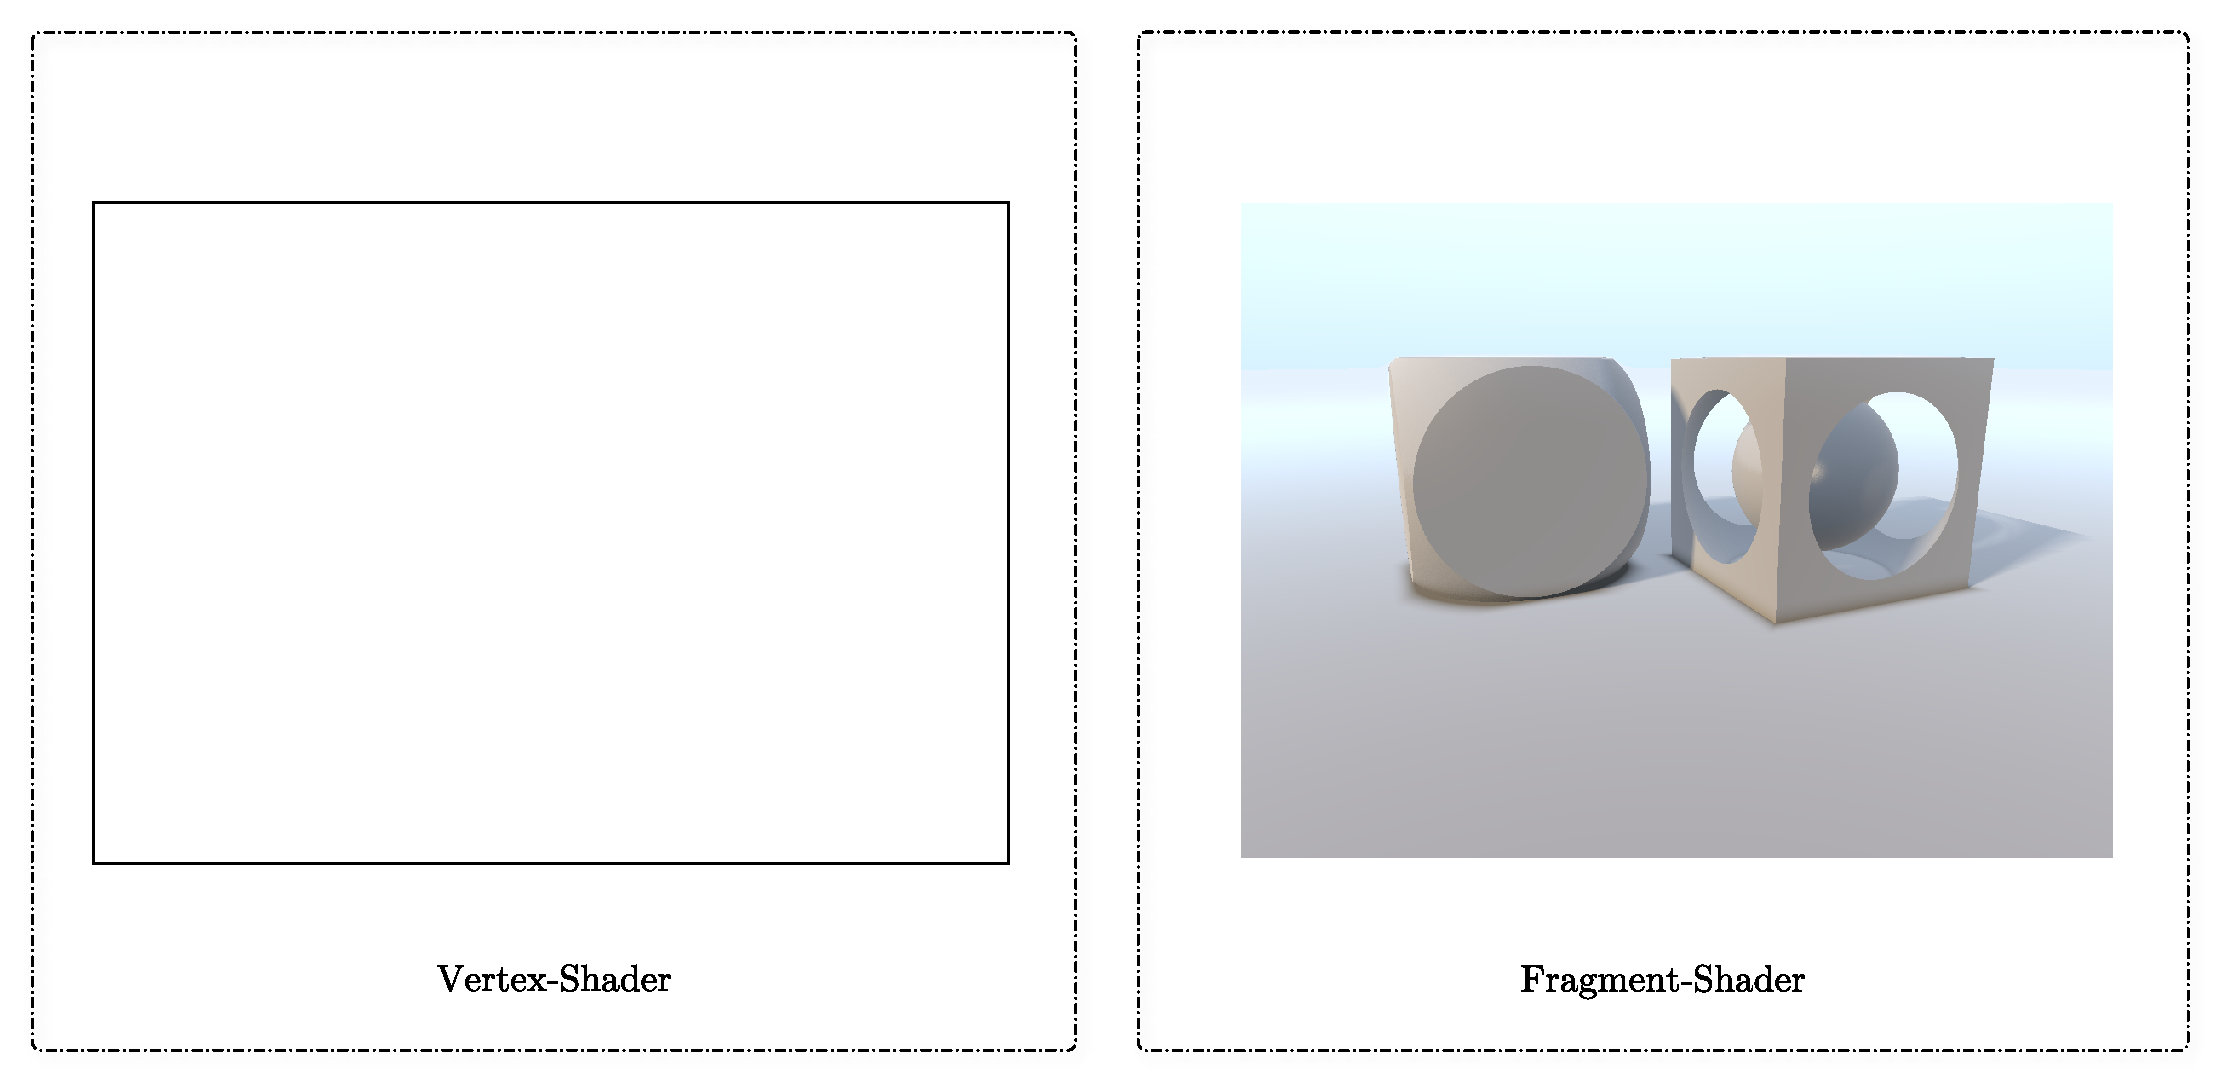
\includegraphics[width=0.8\textwidth]{img/prototype_shaders.pdf}
    \caption{Bildliche Darstellung der Funktionsweise von Vertex- und
        Fragment-Shader der Applikation\protect\footnotemark}\label{fig:prototype_shaders}
\end{figure}
\footnotetext{Eigene Darstellung mittels yEd.}
